
\chapter{Monte Carlo integration methods}
\label{ch:mcmethods}
The application of Monte Carlo techniques in the Statistics domain is increasing popular. In the Bayesian framework, unknown parameters are assumed to be random variables and admit prior distribution that characterises the initial belief. The belief is updated with new observable evidence using Bayes theorem.

More formally, let specify the initial belief of a Bayesian model, $M$ as the prior disitribution $p(\theta \mid M)$, the probability of observing an observation $x$ given the model (likelihood) as $p(x \mid \theta, M)$. Using Bayesin Theorem, the updated belief (posterior distribution) $p(\theta \mid M)$ is given as follows:
\begin{align}
  p(\theta \mid x , M) &= \frac{p(x \mid \theta , M) p(\theta \mid M)}{p(x \mid M)} \nonumber \\
                   &\propto p(x \mid \theta , M) p(\theta \mid M) \label{eq:bayes} \\
  \text{posterior} &\propto \text{likelihood} \times \text{prior}
\end{align}
Whilst the problem formulation is elegant, there remains some subtle issues, e.g., the calculation of normalising constant, the choice of prior, etc. Refer \cite{BD12} for details. The discussion only focuses on how Monte Carlo integration techniques is used to solve some of the issues involved in Bayesian framework.

To calculate the normalisation constant in $p(x \mid M)$ in \eqref{eq:bayes}, we would need to be able integrate the following
\begin{equation}
  p(x \mid M) = \int p (x \mid \theta, M)p(\theta \mid M) d\theta
\end{equation}
analytically which is often not feasible. The Method Carlo integration methods allow one to compute an estimate of this quantity using samples generated from simulation\footnote{Traditionally, the need of normalisation constant is often circumvented by making use of conjugate prior (the choices of certain prior distributions that yield posterior distributions from the same family) in an analytical fashion.}.

The need of calculate the integral of an espression also arise in the marginalisation of nuisance parameter. For example, let $y$ be an nuisance parameter, the marginal density of $x$ can be obtained from the joint density as follows:
\begin{equation}
  p(x \mid y, M) = \int p(x, y \mid M) dy
\end{equation}
If the integral cannot be computed analytically, Monte Carlo integration methods can be used to estimate the quantity of interest.

Another related problem is to calculate the expectation. This often arise when one attempts to summarise the posterior distribution in some way. For example, the expected value of a function of the parameter:
\begin{equation}
  I = E[f(x)] = \int f(x)p(x)dx
\label{eq:int}
\end{equation}
where $f(\cdot)$ is some function of interest, $p(\cdot)$ is the probabilty density function of $x$. Again, this may not have an analytic solution. We may use Monte Carlo integration methods to compute an estimate for this integral.

\section{Perfect Monte Carlo}
In the simplest setting, assuming we are able to sample $N$ independent and identically distributed (i.i.d.) points of $x$ from $p(\cdot)$, denote these as $\{x^i\}$ where $i$ is from $1 \ldots N$, a Monte Carlo estimate of $I$ using the the point masses of the samples is:
\begin{equation}
  \hat{I} = \frac{1}{N} \sum^N_{i=1} f(x^i)
\end{equation}
Informally, this estimate approximates the continous distribution with a discrete distribution with random support. It can be shown that this estimate is unbiased and converge almost surely to $I$ as $N \rightarrow \infty$ (Law of Large number).

If the variance of $f(\cdot)$ is bounded ($\sigma^2_f < \infty$), then the following central limit theorem holds:
\begin{equation}
  \sqrt{N}(\hat{I} - I) \Longrightarrow N(0, \sigma^2_f) \text{ as } N \rightarrow \infty
\end{equation}
where $\Longrightarrow$ denotes convergence in distribution. It is important to note that the converengece rate of $\frac{1}{\sqrt{N}}$ is independent of the dimensions of $x$. This is in constrast with any determinstic method that has a rate that decreases a the integral dimension increases \cite{RCP05}. This is the main advantage of Monte Carlo integration.

\section{Rejection sampling}
However, it is not always possible to sample directly from the distribution $p$. Suppose we can find an instrumental distribution $q$ that is easy to sample from such that $cq(x)$ that dominates $p$ such that $cq(x) \geq p(x) \geq 0$ for all $x$. then to get a random sample from $p$, we can first sample from $q$ instead and accept the sample with acceptance probability $\alpha(x)=\dfrac{p(x)}{cq(x)}$. If the sample is rejected, repeat the process until success. The algorithm is summarised in Algorithm \ref{algo:rejectionsampling}.

\begin{algorithm}
\caption{Rejection Sampling}\label{algo:rejectionsampling}
\begin{algorithmic}[1]
\Function{RejectionSampling}{n}
\State $r = [\ ]$
\Repeat
  \State sample $x \sim q$
  \State sample $u \sim {\cal U}(0,1)$
  \If {$u \leq \dfrac{p(x)}{cq(x)}$}
    \State $r \gets [r,x]$
  \EndIf
\Until{len(r)=n}
\EndFunction
\end{algorithmic}
\end{algorithm}

One could easily see that the optimal choice of proposal distribution $q*$ is that one minimize the area subject to the constraint that it dominates the target density $p$. Unfortunately, in practice a rejection sampling is only feasible in low dimension and then it becomes very ineffective as the dimension increases as lots of samples generated samples woud rejected.

\section{Importance sampling}
Instead of making a binary accept-reject decision on each sample, the main idea behinds important sampling is to weight each sample based on how well the sample from the proposal distribution $q$ resembles the target distribution $p$. More formally, assume we have an instrumental distribution $q$ that is easy to sample from which has support that includes $p$, we can write \eqref{eq:int} as:
\begin{align}
  I &= \int f(x)\dfrac{p(x)}{q(x)}q(x) dx \nonumber \\
    &= \int f(x)w(x)q(x) dx
\end{align}
where $w=\dfrac{p(x)}{q(x)}$, which is commonly known as the importance weight. Based on this reformulation, a possible Monte Carlo estimate of $I$ is given as follows:
\begin{equation}
  \hat{I} = \dfrac{\frac{1}{N} \sum^N_{i=1} w(x^i)f(x^i)}{\frac{1}{N} \sum^N_{j=1} w^j} = \sum^N_{i=1} \tilde{w}^i f(x^i)
\label{eq:is}
\end{equation}
where $\tilde{w}^i=\displaystyle\sum^N_{i=1}\dfrac{w^i}{\sum^N_{j=1}w^j}$ is the normalised importance weight. This estimate is biased as it uses the ratio of two estimator but it is still asymtoptically consistent.

\section{Markov chain Monte Carlo (MCMC)}
%The rejection and importance algorithms scale badly with dimensionality. In some problems, it may still possible to decompose the probability distribution of interest, $P(x_{1:N})$ into low dimensional conditional distributions and proceed from there. However, this is not often feasible in practice.

Markov chain Monte Carlo (MCMC) are a set of algorithms that allows ones to draw random samples from the target probability distribution by constructing a ergotic Markov chain process which has its stationary distribution set to be target desired distribution. 

\subsection{Markov Chain}
Conceptually, Markov chain is a stochastic process in which the past and future states of the process are independent given the current state. A Markov chain can be viewed as an \emph{ordered} sequence of states $\{x_{1:N}\}$, in which state $x_t$ only depends on state $x_{t-1}$, i.e., the state at time $t$ is determined based on some trasition distribution of the form $p(x_t \mid x_{t-1})$, which is independent of all previous states $x_{t-2}, x_{t-3}, \ldots$. 

To ensure the Markov chain converges to a steady state (stationary distribution), the chain needs to satisfy the following properties:
\begin{enumerate}
\item irreducible --- no matter where it starts a chain, it is possible to reach all other states in finite amount time steps.
\item aperiodic --- 	for all the states $i$, the chain can  return to state $i$ at irregular time.
\item positive recurrent --- for all the state $i$, the chain will definitely revisit the state in finite amount time stpes.
\end{enumerate}

In practice, it is usually not difficult to construct the required Markov Chain, the more difficult problem is to determine how many steps it takes to converge, often known as mixing. Various visual diagnostic have been developed, yet it is often a matter of art. Refer \cite{RCP05} for details.

In the following sections, we present two basic MCMC algorithms: Metropolis Hastings algorithms, Gibbs algorithms and a third algorithm in which these two basic algorithms are ``mixed and matched'' in a hierarchical fashion to form a more advanced samplers to fit application needs.

\subsection{Metropolis-Hastings sampling}
The first major MCMC algorithm was devised by Metropolis in \cite{MN53}. The algorithm constructs a Markov Chain by proposing a random walk step based a proposal distribution is symmetric, i.e., the probability of moving from state $t$ to state $t-1$ is the same as the probability of moving from state $t-1$ to state $t$ ($q(x_{t} \mid x_{t-1}) = q(x_{t-1} \mid x_{t}$). The proposed step is then either accepted or rejected according to an acceptance probability, $\alpha(x)= \min\left(1, \dfrac{p(x_t)}{p(x_{t-1})}\right)$, where $p(x)$ is the target probability density evaluated at $x$.

This algorithm was generalised by Hastings \cite{WKH70} to allow the use of non-symmetric proposal density, with an adjustment to the accenptance probability $\alpha(x) = \min\left(1, \dfrac{p(x_t)q(x_t \mid x_{t-1})}{p(x_{t-1})q(x_{t-1} \mid x_{t})}\right)$ and hence the name, Metropolis-Hastings sampling. This algorithm is summarised in Algorithm \ref{algo:metropolishastings}.

\begin{algorithm}
\caption{MetropolisHastings}\label{algo:metropolishastings}
\begin{algorithmic}[1]
\Function{MetropolisHastings}{n}
\State $r = [\ ]$
\Repeat
  \State sample $x_t \sim q(x_{t-1})$
  \State sample $u \sim {\cal U}(0,1)$
  \If {$u \leq \min\left(1, \dfrac{p(x_t)q(x_t \mid x_{t-1})}{p(x_{t-1})q(x_{t-1} \mid x_{t})}\right)$}
    \State $x_{t-1} \gets x_{t}$
    \State $r \gets [r,x_{t-1}]$
  \EndIf
\Until{len(r)=n}
\EndFunction
\end{algorithmic}
\end{algorithm}

It is not hard to see that the algorithm works best if the density $q$ matches the shape as density $p$, which is often unknown. Assuming a Gaussian proposal density $q$ is used, there is also an addtional parameter, namely the variance $\sigma^2$ is required to be tuned. There is a trade-off to be made in the tuning process. If the $\sigma^2$ is set too be too small, the chain is likely to mix slowly (i.e., the proposed step is likely to be accepted yet each successive move is very slow and therefore the chain will converge to target distribution $p$ at a slow rate). On the other hand, if $\sigma^2$ is too large, the proposed step is likely to be rejected as it is likely to hand in a region of much lower probability density and the chain will converge slowly again. Again, refer \cite{RCP05} for details on convergence dianogstic.

\subsection{Gibbs sampling}
Gibbs sampling \cite{GS84} is a special form of the Metropolis–Hastings sampling. The key idea in Gibbs sampling is to re-write the target multivariate distribution of interest as a product of conditional probability distributions of lesser number of parameters. A Markov Chain is then constructed to generate samples for each parameter \emph{in turn} from the conditional distributions with an acceptance rate $\alpha(x)=1$, i.e., accept all the samples.

More formally, suppose we would like to have obtain $k$ samples of $\mathbf{x}=(x_1,x_2,\ldots, x_n)$ from $p(x_1, \ldots, x_n)$, assuming we start with an initial value $\mathbf{x}^{0}$. For each sample $(\mathbf{x}^{i}: i \in \{1 \dots n\})$, sample $x_j^{(i)}$ from the conditional distribution $p(x_j|x_1^{(i)},\dots,x_{j-1}^{(i)},x_{j+1}^{(i-1)},\dots,x_n^{(i-1)})$. In other words, sample each variable from the distribution of that variable conditioned on all other variables, making use of the most recent values and updating the variable with its new value as soon as it has been sampled. The algorithm is summarised in Algorithm \ref{algo:gibbs}.

\begin{algorithm}
\caption{Gibbs}\label{algo:gibbs}
\begin{algorithmic}[1]
\Function{Gibbs}{n}
\State $r = [\ ]$
\State sample $x^{(0)}$
\Repeat
  \State sample $x^{(t)} \sim p(x_j|x_1^{(i)},\dots,x_{j-1}^{(i)},x_{j+1}^{(i-1)},\dots,x_n^{(i-1)})$
  \State $r \gets [r,^{t}]$
\Until{len(r)=k}	
\EndFunction
\end{algorithmic}
\end{algorithm}

There are variations of Gibbs sampling techniques. For examples, a blocked Gibbs sampling groups more than one variables and sample from the joint distribution conditioning on other variables. Refer \cite{RCP05} for details. 

\section{Hidden Markov Models}
Hidden Markov Models (HMMs) is a class of models that have been applied to many different problems in statistics, signal processing and engineering. Many Monte Carlo techniques have been developed to deal with inference in HMMs, one of which that we have paricular interest in is the Sequential Monte Carlo (SMC). This section provides a brief background on HMMs that is essentially to understand SMC. Refer \cite{CO05} for further details of inference techniques for HMMs in general.

HMMs can be viewed as a class of models that consist of two related process: an underlying Markov process, $X_t$, which is the target process of interest, and a observable process, $Y_t$, which its state can be measured and therefore provides some information about $X_t$. Moreover, it is assumed that these two processes also have conditional independence properties as shown using the graphical model representation in Figure \ref{fig:HMM}. More formally, these properties can be summarised as follows:
\begin{align}
   \Pr(X_n \mid X_{1:n}) &= \Pr(X_{n-1})   \nonumber \\
   \Pr(Y_n \mid X_{1:n}  &= Y_{1:n}) = \Pr(Y_n \mid X_{1:n}) 
	1 + 1 conditional indepednent
\end{align}

\begin{figure}
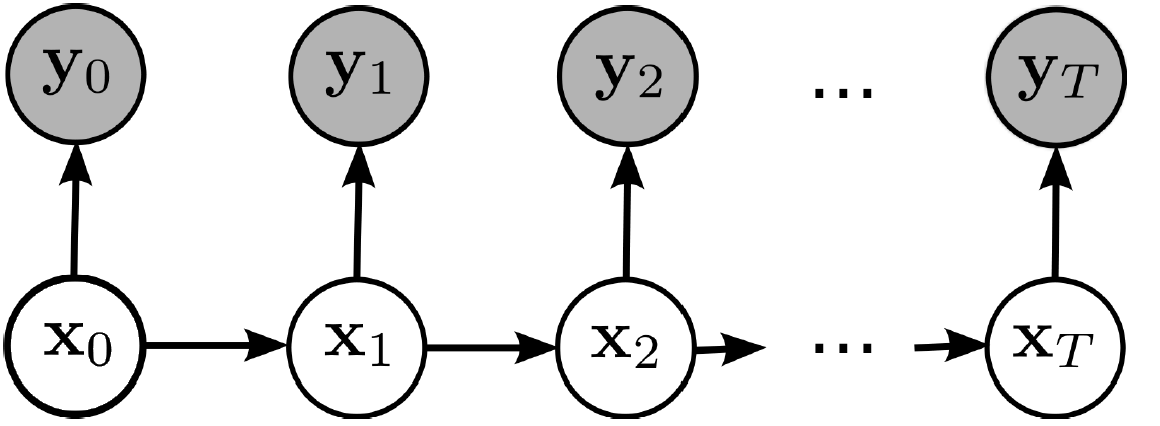
\includegraphics[scale=1]{hmm.png} 
\caption{Hidden Markov Models}
\label{fig:HMM}
\end{figure}

It is worth emphasizing here that this model is designed to capture systems that evolve from one state to another over time, generating observation after each state move. The inference problem is typically about estimating the state(s) in \emph{real-time} given the observations. This imposes an implicit requirement from the computation perspective that the estimate calculation cost should remain constant over time (i.e., the calculation cost does not increase with the increasing number of states).

Arguably, the most common inference problem in HMMs is the smoothing distribution, $p(x_{1:t} \mid y_{1:t})$, that is estimating the states $x_{1:t}$ based on the sequence of observations up to time $t$, $y_{1:t}$. Using Bayes rules, we can write the density of the distribution of interest as follows:
\begin{align}
    p(x_{1:t} \mid y_{1:t}) \propto p(x_{1:t} \mid y_{1:t-1}) g(y_t \mid x_t) \nonumber \\
    p(x_{1:t} \mid y_{1:t-1})f(x_t \mid x_{t-1})g(y_t \mid x_t)
\end{align}
where $f(x_t \mid x_t=1)$ is the transition density and $g(y_t \mid x_t)$ is the likelihood. This recursion is often re-written into two separate steps: prediction (the estimation of distribution of $t$ states given only $t-1$ states) and update steps (the correction of the predicted distribution taking into account the new observation as follows:
\begin{align}
  p(x_{1:t} \mid y_{1:t-1}) &= p(x_{1:t-1} \mid y_{1:t-1})f(x_t \mid x_{t-1}) \nonumber \\
  p(x_{1:t} \mid y_{1:t})   &= \dfrac{p(x_{1:t} \mid y_{1:t-1}) g(y_t \mid x_t)}{\int p(x_{1:t} \mid y_{1:t-1}) g(y_t \mid x_t) dx_{1:t}}
\end{align}
Moreover, the estimate of any smoothing distribution $p(x_{j:k} \mid y_{1:t})$ where $j \leq k \leq l)$ can be obtained by integrating out $x$ that are not interested in as follows:
\begin{equation}
  p(x_{j:l} \mid y_{1:t}) = \int p(x_{1:t} \mid y_{1:t}) dx_{1:j, l+1:t}
\label{eq:smoothing}
\end{equation}
One particular smoothing distribution of interest is the final marginal distribution $p(x_t \mid y_{1:t})$, which is often referred to as the filtering distribution.

Another distribution of interest is  the prediction distribution, that is the estimation of the distribution of any unseen \emph{future} state based on the sequence of observations up to time. Referring to \eqref{eq:smoothing}, if we let $j = 1$ and $l \geq n$ in , we have:
\begin{equation}
  p(x_{j:l} \mid y_{1:t}) = p(x_{j:t} \mid y_{1:t}) \prod^k_{i=t+1} f(x_i \mid x_{i-1})
\end{equation}
Therefore, any prediction density can be obtained by integrating out the variables of not interest from the above equation.

The problem of distribution estimation as discussed appears to be simple, but the problem is in fact far from being resolved in practice. The integral appear in the above equations are often intractable and can only be estimated.

\subsection{Kalman Filter}
In a special case setting, in which the transition distribution of $X_t \mid X_{t-1}$ and the likelihood are Gaussian distributions centred at a point of a linear combination of the conditional variables of the following form:
\begin{align}
  f_n(x_n \mid x_{n-1}, u_n) &= N(A_n x_{n-1} + F_n(u_n), B_n B^T_n) \nonumber \\
  g_n(y+n \mid x_n, u_n)    &= N(C_n x_n{n-1}, D_nD^T_n)
\end{align}

Using the properties of Gaussian distribution, the integral can be resolved analytically. This leads the widely used \emph{Kalman Filter} \cite{KGE60}, which has the following recursion forms:
\begin{align}
  1+1
\end{align}
There are various extensions to this approach. For example, the Extended Kalman Filtre (EKF) which uses Taylor Series expansion to linearise at the conditional variables locally, Unscentend Kalman Filter, etc.. Refer \cite{WG95} for further details on Kalman Filter.

\section{Sequential Monte Carlo}
As mentioned, there is however no analytical solution for this estimation problem in a general settings for this model. A common  technique to dealing with this problem is Sequential Monte Carlo (SMC). Conceptually, the distribution of a state at any point of time is represented using a set of weighted samples (a.k.a. particles). These particles are propagate from one state to another through time by proper re-weighting and re-sampling as necessary to track the changes of the distribution. To estimate the smoothing/filtering/prediction distribution, the integrals are performed on these samples using Monte Carlo technique in a recursion fashion, i.e., the estimation problem at step $t$ is calculated with the estimate obtained at time $t-1$, hence the name.

\subsection{Sequential Important Sampling (SIS)}

\subsection{Sequential Important Resampling (SIR)}

\subsection{Parameter estimation}


\section{Conclusion}
In this chapter, 
